\documentclass{article}
\usepackage[left=2cm,right=2cm,top=2cm,bottom=2cm]{geometry}
\usepackage[utf8]{inputenc}
\usepackage[german]{babel}
\usepackage{amsmath}
\usepackage{dsfont}
\usepackage[export]{adjustbox}
\usepackage{amsthm}
\usepackage{color}
\usepackage{amsfonts}
\usepackage{amssymb}
\usepackage{wasysym}
\usepackage{makeidx}
\usepackage{graphicx}
\usepackage[colorlinks=true,urlcolor=blue,linkcolor=blue]{hyperref}
\usepackage{ziffer}
\usepackage{minted}
\usepackage{xcolor}
\usepackage{framed}
\usepackage{mdframed}
\usepackage{subfiles}
\usemintedstyle{emacs}

\definecolor{purp}{HTML}{9A72AC}
\definecolor{re}{HTML}{FC6255}
\definecolor{gre}{HTML}{83C167}
\definecolor{blu}{HTML}{58C4DD}
\definecolor{shadecolor}{rgb}{0.85,0.85,0.85}
\definecolor{bg}{rgb}{0.95,0.95,0.95}
\setlength{\parindent}{0em} 

\BeforeBeginEnvironment{minted}{\begin{mdframed}[linewidth =2 ,backgroundcolor=bg , linecolor=black, linewidth=0.5]}
\AfterEndEnvironment{minted}{\end{mdframed}}

\newtheorem{defi}{Definition}
\BeforeBeginEnvironment{defi}{\begin{mdframed}[linewidth =2 ,backgroundcolor=bg , linecolor=black, linewidth=0.5]}
\AfterEndEnvironment{defi}{\end{mdframed}}

\newcommand{\bsp}{\textbf{Beispiel}:}
%\newcommand{\task}{\textbf{Aufgabe}:}

\newcommand{\bol}[1]{\textbf{#1}}
\newcommand{\q}[1]{\glqq #1\grqq}
\newcommand{\DODO}[1]{\textbf{\textcolor{red}{DODO:}} #1 \\ \begin{center}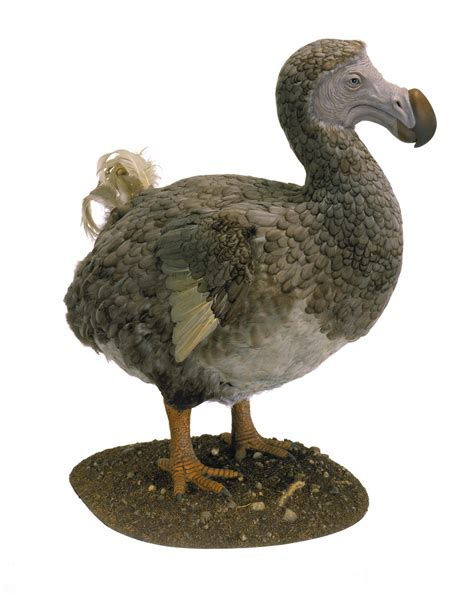
\includegraphics[scale=0.2]{../../media/dodo.jpg} \end{center}}

\newenvironment{task}[1]{
    \begin{shaded*}
    \textbf{Aufgabe #1}:
}{
    \end{shaded*}
}


\begin{document}

\subsection{Ein erster Ansatz}

Wir beginnen wie bei den Listen zunächst mit einem naiven Ansatz (d.h. noch ohne Compositum). Der grundlegende Aufbau entspricht dem der Liste, nur hat jeder Knoten zwei mögliche Nachfolger, die im Folgenden links bzw. rechts (left bzw. right) genannt werden. In Anlehnung an die Einleitung beschränken wir uns zunächst auf Zahlen als Werte und verzichten auf eine Mensch- oder Datenelementklasse. Eine weitere, häufig nützliche Eigenschaft ist, dass nach dem Einfügen jeder Wert nur einmal im Suchbaum vorkommt. \\
\textbf{Randnotiz}: In der Mathematik hat eine Menge die Eigenschaft, dass keine Elemente doppelt vorkommen (Englisch: set). Auch in der Informatik kann diese Eigenschaft nützlich sein. Unser Suchbaum wird eise Eigenschaft erfüllen. Java bietet natürlich auch schon eingebaute Strukturen mit ähnlichen Eigenschaften. Diese und weitere Mengeneigenschaften sind im \href{https://docs.oracle.com/javase/7/docs/api/java/util/Set.html}{Set}-Interface zusammengestellt.
\begin{center}
    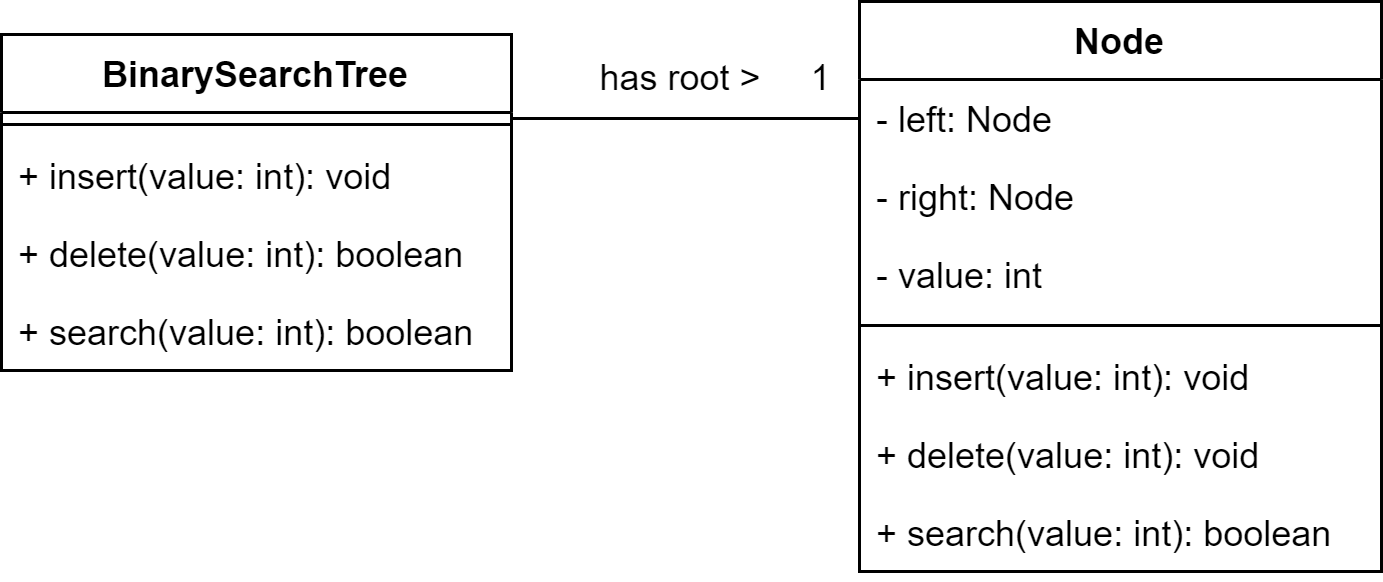
\includegraphics[scale=0.25]{../media/bin_tree_basic.png}
\end{center}
\textit{Hinweis:} Die üblichen getter- und setter-Methoden wurden im Klassendiagramm der Übersichtlichkeit halber weggelassen. \\
Die Klassenrümpfe sehen damit wie folgt aus:
\begin{minted}{Java}
    public class BinarySearchTree {
        private Node root;

        public void insert(int toInsert) {
            // ... 
        }

        public void delete(int toDelete) {
            // ...
        }

        public boolean search(int toSearch) {
            // ...
        }
    }

    public class Node {
        private Node left;
        private Node right;
        private value; 

        public Node(int value) {
            this.value = value;
        }

        //...
    }
\end{minted}
Wie immer besteht bei der Implementierung der Konstruktoren Spielraum, so könnte man z.B. bei Erzeugung eines neuen Baumes bereits einen Wert als Wurzel fordern. \\
Wir beginnen mit der Einfügen-Methode:
\begin{minted}{Java}
    //class BinarySearchTree 
    public void insert(int toInsert) {
        if(root == null) {
            root = new Node(toInsert);
        } else {
            root.insert(toInsert);
        }
    }

    //class Node
    public void insert(int toInsert) {
        //Ist der Wert schhon vorhanden brechen wir ab
        if(toInsert == value) {
            return;
        }
        if(toInsert < value) {
            // Ist der einzufügende Wert kleiner fügen wir im linken Teilbaum ein
            if(left != null) {
                left.insert(toInsert);
            } else {
                left = new Node(toInsert);
            }
        } else {
            //Andernfalls im rechten Teilbaum
            if(right != null) {
                right.insert(toInsert);
            } else {
                right = new Node(toInsert);
            }
        }
    }
\end{minted}

Da die Löschen-Methode deutlich schwerer zu implementieren ist als die Suchen-Methode beginnen wir mit dieser:

\begin{minted}{Java}
    //class BinarySearchTree 
    public boolean search(int toSearch) {
        if(root == null) {
            return false;
        } else {
            return root.search(toSearch);
        }
    }

    //class Node 
    public boolean search(int toSearch) {
        if(toSearch == value) {
            return true;
        } else if(toSearch < value) {
            if(left == null) {
                return false;
            } else {
                return left.search(toSearch);
            }
        } else {
            if(right == null) {
                return false;
            } else {
                return right.search(toSearch);
            }
        }
    }
\end{minted}
Die Struktur ist - abgesehen vom Vergleich mit dem Wert des derzeitigen Knotens - analog zur Einfügen-Methode. Das überrascht nicht, da wir für die Suche denselben Weg laufen, den das Element auch beim Einfügen genommen hätte. \\
Möchte man ein Element entfernen, so muss wie bei der Liste neu verzeigert werden. Dies gestaltet sich aber deutlich schwieriger, da nicht einfach zum nächsten Element verzeigert werden kann (zumindest nicht notwendigerweise), außerdem muss die Sortierung sichergestellt werden. Man muss drei Möglichkeiten unterscheiden:
\begin{itemize}
    \item \textbf{Der Knoten ist ein Blatt} - er hat also keine Kinder und kann einfach entfernt werden.
    \item \textbf{Der Knoten hat nur ein Kind} - das Kind kann als neuer nächster (links oder rechts) verzeigert werden.
    \item \textbf{Der Knoten hat zwei Kinder} - in diesem Fall gilt die Regel: \q{entferne den kleinsten Wert aus dem rechten Teilbaum und setze ihn an diese Stelle}.
\end{itemize}

Die Umsetzung dieser Regeln soll auf eine spätere Gelegenheit verschoben werden.

\begin{task}{für Experten}
    Implementiere die Entfernen(int zuEntfernen)-Methode (delete(toDelete)).
\end{task}

Zunächst zu einer drängenderen Frage:
\begin{center}
    \textbf{Wie gibt man die Werte eines Baumes sinnvoll aus?}
\end{center}

\subsection{Die Traversierung eines sortierten Suchbaumes}

Bei Listen ergibt sich eine \q{natürliche} Möglichkeit der Ausgabe - einfach ein Element nach dem anderen. Bei Bäumen gestaltet sich dies schon schwieriger, man könnte an der Wurzel beginnen, aber soll dann zuerst der linke - oder doch der rechte Knoten besucht werden? Und wenn man zum linken Teilbaum geht, geht es dann im linken Teilbaum weiter, oder wechselt man zum rechten Teilbaum über? \\
Auf diese Fragen gibt es keine eindeutige Antwort, es gibt viele gleichberechtigte Methoden, einen Baum zu durchlaufen (zu \textbf{traversieren}). Wir beschränken uns im Folgenden auf drei Möglichkeiten:

\begin{enumerate}
    \item \textbf{Pre-Order (NLR)}
    \item \textbf{In-Order (LNR)}
    \item \textbf{Post-Order (LRN)}
\end{enumerate}
Alle drei Möglichkeiten arbeiten rekursiv und durchlaufen den Baum vollständig, lediglich die Position der Ausgabe des Wertes des Knotens ändert sich. (Die Bedeutung der Abkürzungen wird im weiteren Verlauf klar)
\subsubsection{Pre-Order}
In dieser Methode werden zunächst die Daten des aufgerufenen Knotens ausgegeben, dann wird die Methode auf dem linken Kind aufgerufen, zuletzt auf dem rechten Kind. Ein Beispiel:
\begin{center}
    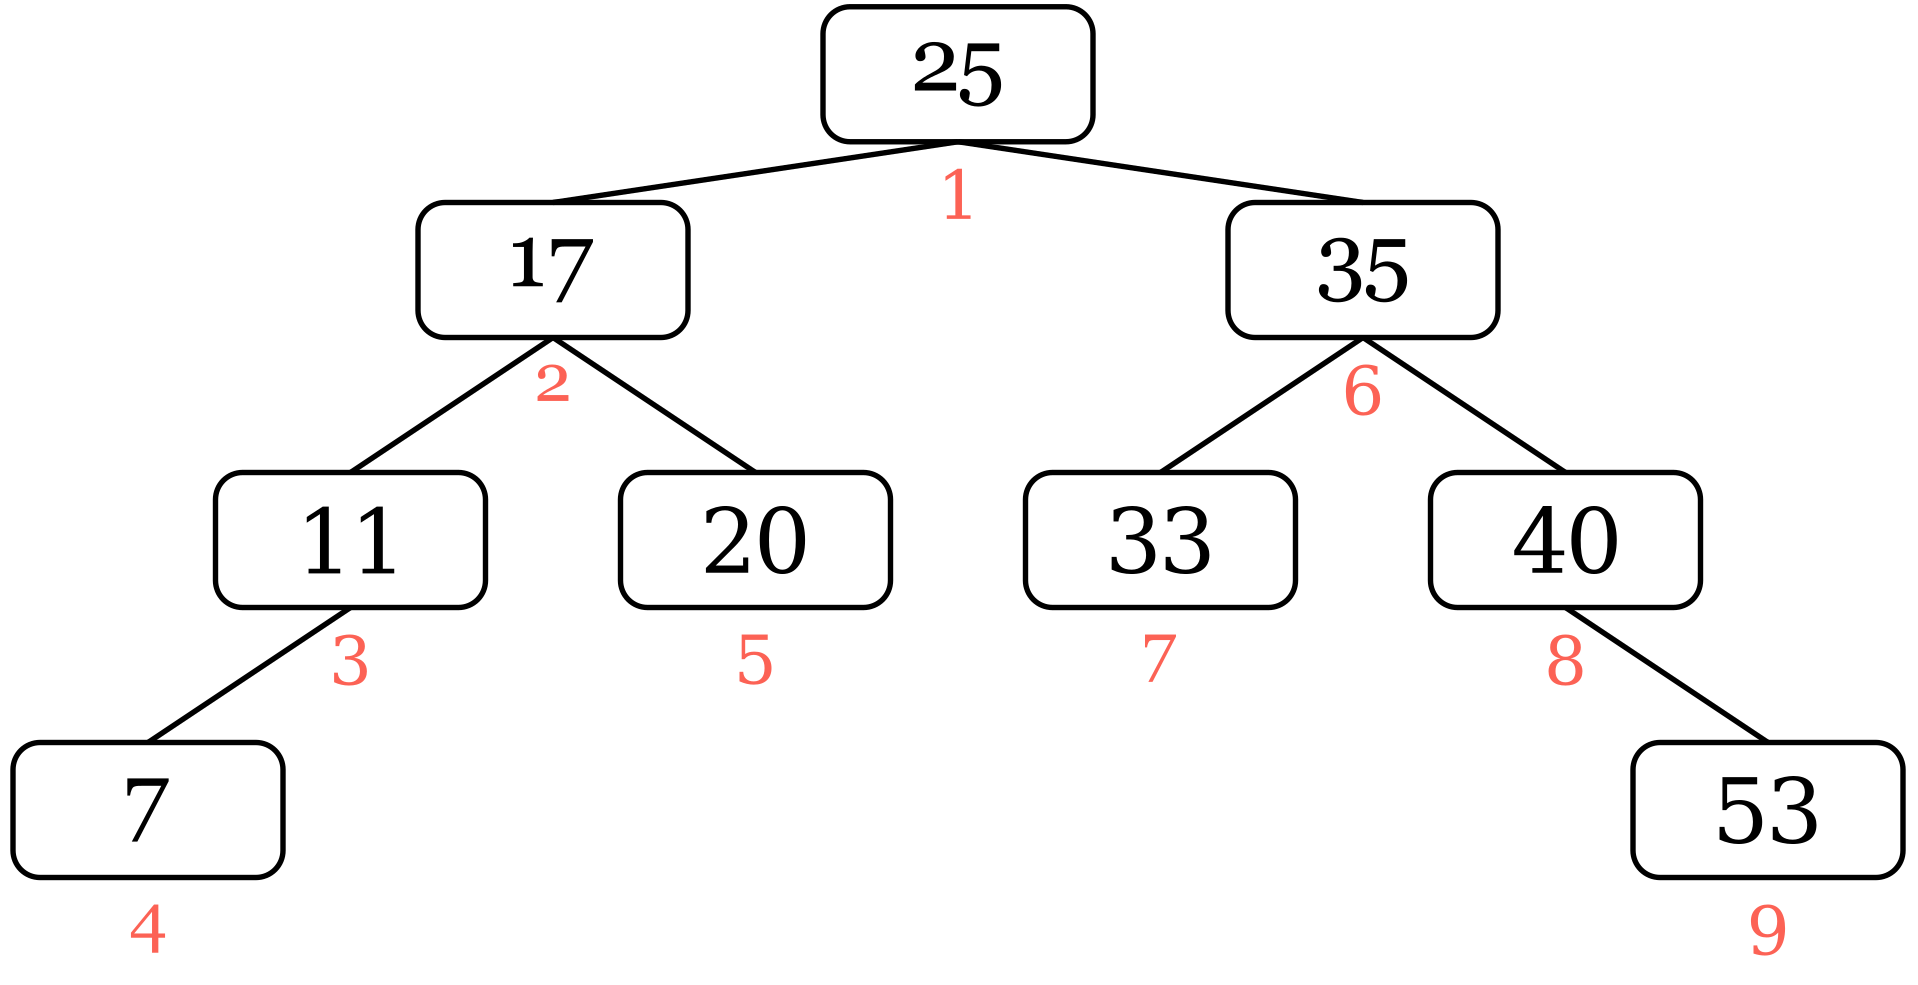
\includegraphics[scale=0.2]{../media/preorder.png}
\end{center}
Auf der Wurzel $25$ wird die printPreOrder-Methode aufgerufen. Die Wurzel gibt ihre Daten aus und ruft anschließend auf dem linken Kind $17$ printPreOrder auf. Die $17$ gibt nun ihrerseits ihren Wert aus und gibt den Aufruf an die $11$ aus, nach der Ausgabe der $11$ folgt der Aufruf und die Ausgabe von $7$. \\
Da $7$ aber keine weiteren Kinder hat, erfolgt auch kein weiterer Funktionsaufruf, es wird also zurück zur $11$ gesprungen. Da diese aber auch kein rechtes Kind hat, kann dort nicht weiter aufgerufen werden und die Ausführung kehrt zur $17$ zurück (mit zurückkehren ist damit natürlich nur gemeint, dass wir den nächsten Funktionsaufruf auf dem Knoten $17$ durchführen, es muss nicht \q{gessprungen} werden, da nur ein Stapel an Funktionsaufrufen abgearbeitet wird). \\
Da die $17$ einen rechten Nachbarn hat, wird die Methode auf dem rechten Nachbarn $20$ aufgerufen. Damit ist der linke Teilbaum abgeschlossen und der rechte Teilbaum wird analog ab der 35 abgearbeitet. Insgesamt ergibt sich also:
\begin{center}
    $25 \rightarrow 17 \rightarrow 11 \rightarrow 7 \rightarrow 20 \rightarrow 35 \rightarrow 33 \rightarrow 40 \rightarrow 53$
\end{center}
Eine mögliche Implementierung der Methode mit dem Gerüst aus dem vorherigen Kapitel: 
\begin{minted}{Java}
    //class BinarySearchTree
    public void printPreOrder() {
        if(root != null) {
            root.printPreOrder();
        }
    }

    //class Node 
    public void printPreOrder() {
        System.out.println(value + " ");
        if(left != null) left.printPreOrder();
        if(right != null) right.printPreOrder();
    }
\end{minted}
Alternativ zur direkten Ausgabe auf der Konsole können die Werte auch in einem String zwischengespeichert werden und dieser am Ende zurückgegeben werden. 

\subsubsection{In-Order}
Im Unterschied zur Pre-Order-Variante wird hier zunächst der Aufruf auf dem linken Kind gestartet, ist dieser beendet werden die eigenen Daten ausgegeben, am Ende folgt dann der Aufruf auf dem rechten Kind. In unserem Beispiel ergibt sich damit die folgende Reihenfolge:
\begin{center}
    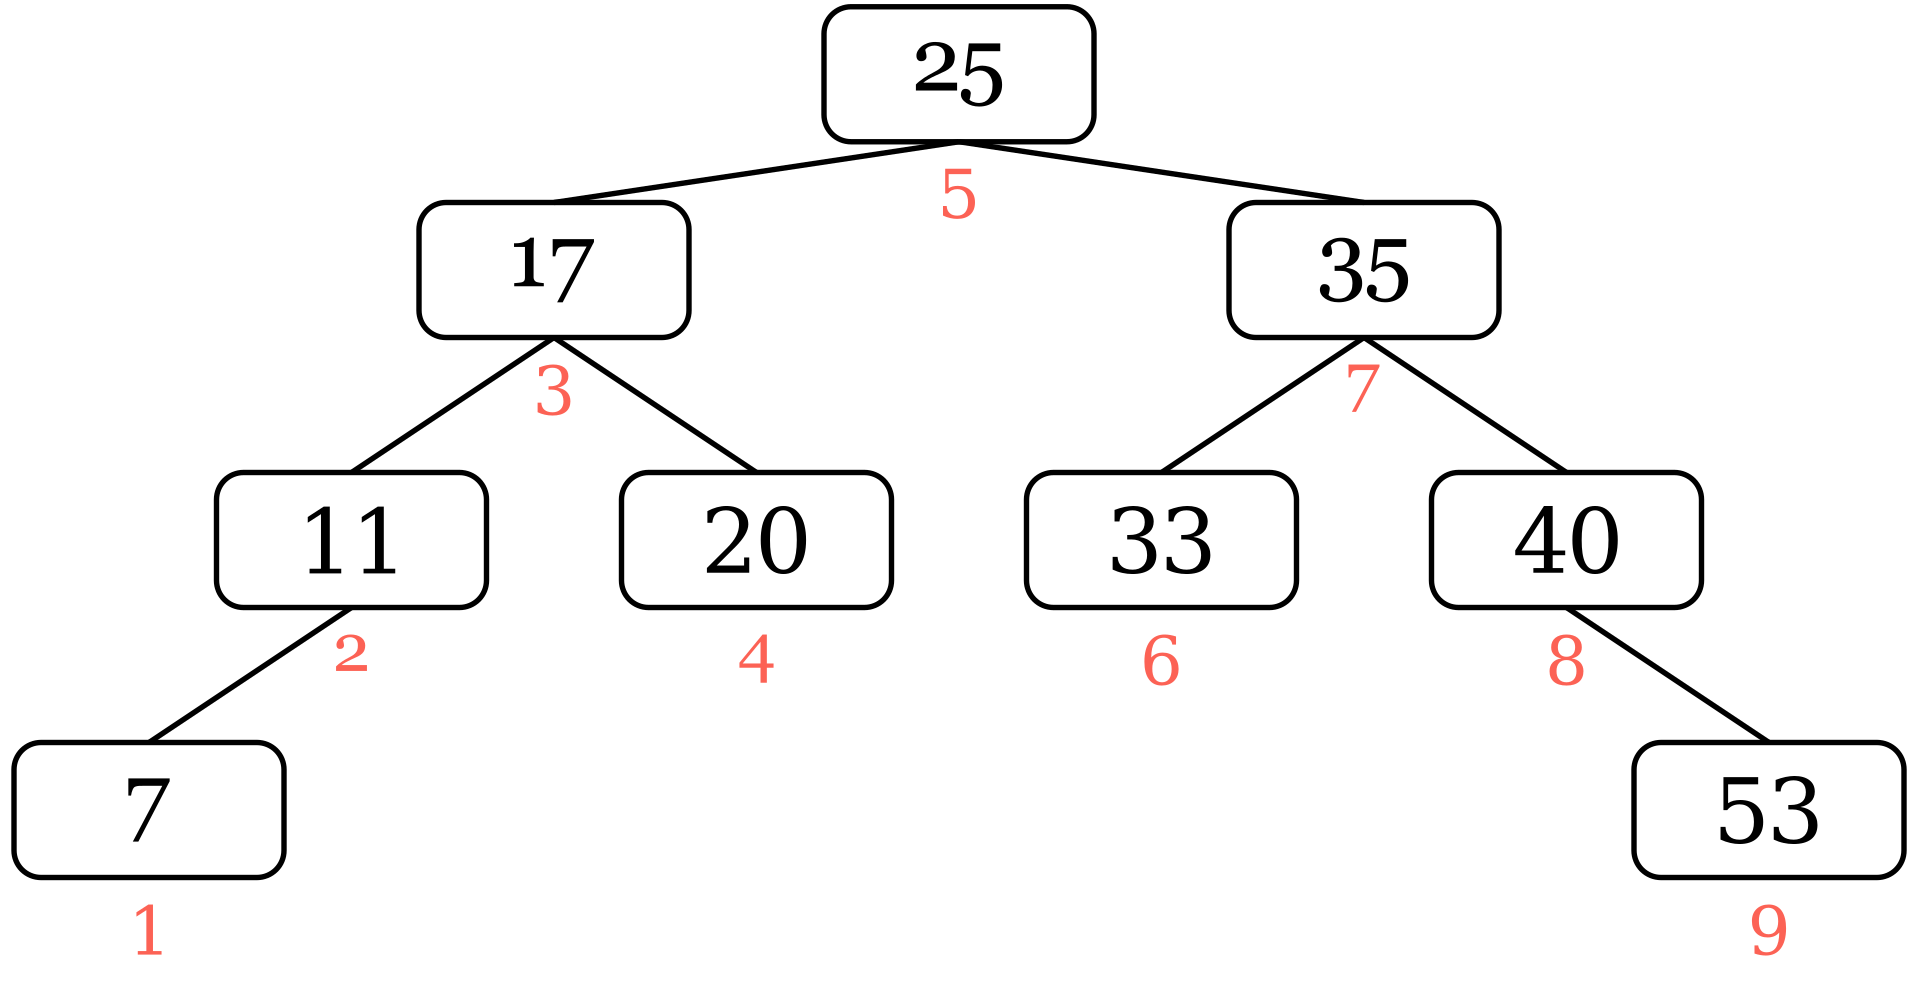
\includegraphics[scale=0.2]{../media/inorder.png}
\end{center}
Da immer zuerst auf dem linken Kind aufgerufen wird, beginnt der Durchlauf \q{links unten} im Baum, in diesem Fall bei der $7$. Nach dem linken Kind wird die eigene Information ausgegeben, weswegen die $11$ folgt. Da es kein rechtes Kind der $11$ gibt wird als nächstes die $17$ ausgegeben, danach deren rechtes Kind, die $20$. Damit ist der linke Teilbaum abgearbeitet und die Wurzel wird ausgegeben. Es folgt wieder analog der rechte Teilbaum. \\
\textit{Hinweis:} Auch im rechten Teilbaum wird \q{links unten} begonnen - dank der rekursiven Natur des Baumes können wir jeden Teilbaum wie einen vollwertigen Baum behandeln! \\
Insgesamt:
\begin{center}
    $7 \rightarrow 11 \rightarrow 17 \rightarrow 20 \rightarrow 25 \rightarrow 33 \rightarrow 35 \rightarrow 40 \rightarrow 53$
\end{center}
Die Implementierung sieht nahezu identisch aus, es hat sich lediglich die Position der Ausgabe verändert: 
\begin{minted}{Java}
    //class BinarySearchTree
    public void printInOrder() {
        if(root != null) {
            root.printInOrder();
        }
    }

    //class Node 
    public void printInOrder() {
        if(left != null) left.printInOrder();
        System.out.println(value + " ");
        if(right != null) right.printInorder();
    }
\end{minted}

\subsubsection{Post-Order}
Bei der Post-Order-Variante werden zuerst beide Kinder (links dann rechts) abgearbeitet, bevor die eigenen Daten ausgegeben werden. In unserem Beispiel: 
\begin{center}
    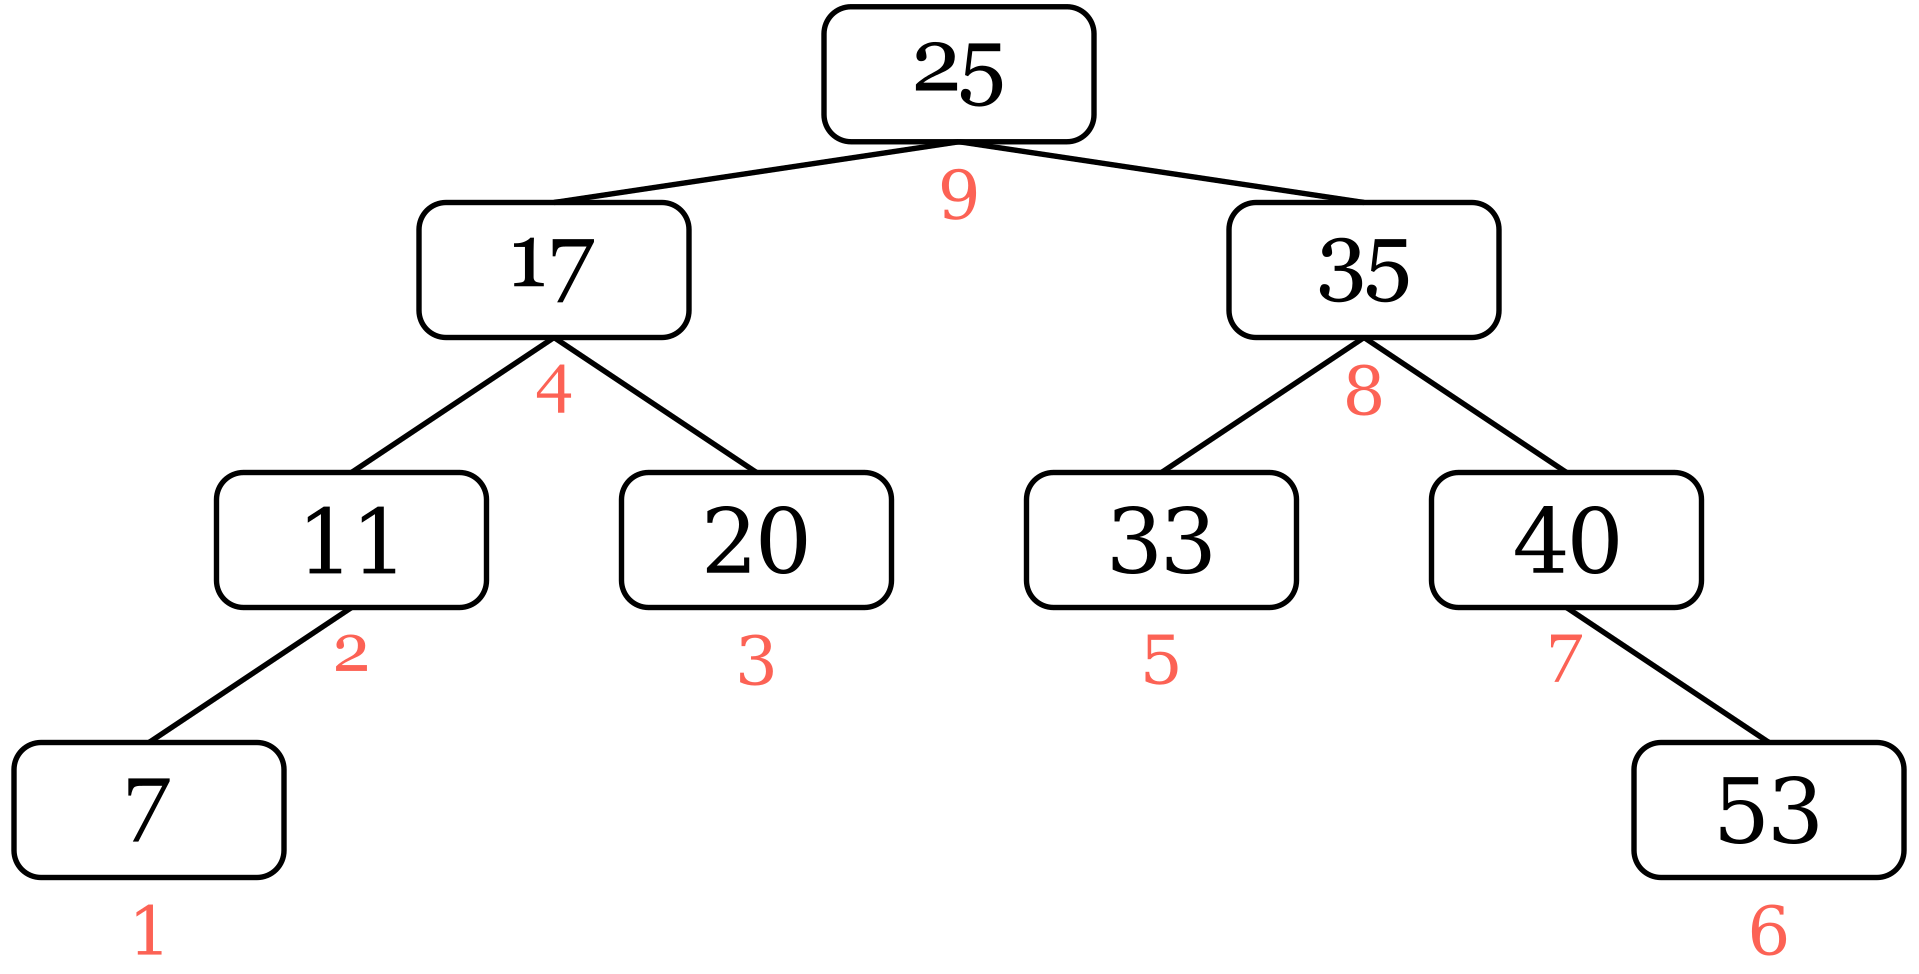
\includegraphics[scale=0.2]{../media/postorder.png}
\end{center}
Der Startpunkt ist wie zuvor die $7$ und da die $11$ kein rechtes Kind hat, ist sie die zweite Zahl. Danach ist jedoch die $20$ als rechtes Kind der $17$ vor dieser an der Reihe. Die Wurzel wird ausgelassen (hier sind wir gestartet, d.h. die Ausgabe erfolgt erst ganz am Ende, nach Abarbeitung des linken und rechten Teilbaums!). Der rechte Teilbaum wird wieder analog abgearbeitet und es ergibt sich:
\begin{center}
    $7 \rightarrow 11 \rightarrow 20 \rightarrow 17 \rightarrow 33 \rightarrow 53 \rightarrow 40 \rightarrow 35 \rightarrow 25$
\end{center}
Im Code:
\begin{minted}{Java}
    //class BinarySearchTree
    public void printPostOrder() {
        if(root != null) {
            root.printPostOrder();
        }
    }

    //class Node 
    public void printPostOrder() {
        if(left != null) left.printPostOrder();
        if(right != null) right.printPostOrder();
        System.out.println(value + " ");
    }
\end{minted} 

\subsubsection{Zusammenfassung und Ausblick}

Da die drei Methoden so ähnlich aussehen, bietet es sich an, sie zusammenzufassen und mit einem \q{Schalter} den Ort der Ausgabe umzuschalten. Dieser Schalter könnte einfach ein String sein, der z.B. auf \q{Post} oder \q{In} verweist. In diesem Fall kann die Funktion aber auch mit einem beliebigen anderen String als Übergabeparameter aufgerufen werden und wir müssen mit diesen Eingaben umgehen.  \\
Um dieses Problem zu umgehen können wir auf eine spezielle Art von Klasse genannt \textbf{Enum} zurückgreifen. In einer solchen Klasse wird ausschließlich eine Liste an nicht veränderbaren Variablen, d.h. Konstanten definiert, die in anderen Klassen verwendet werden können. In unserem Fall könnte das Ganze so aussehen: 
\begin{minted}{Java}
    //enum Order 
    public enum Order {
        PRE,
        POST, 
        IN
    }

    //class BinarySearchTree 
    public print(Order order) {
        if(root != null) {
            root.print(order);
        }
    }

    //class Node
    public void print(Order order) {
        if(order == Order.PRE) System.out.print(value + " ");
        if(left != null) left.print(order);
        if(order == Order.IN) System.out.print(value + " ");
        if(right != null) right.print(order);
        if(order == Order.POST) System.out.print(value + " ");
    }
\end{minted}

In dieser Implementierung wird auch noch einmal schön der Hintergrund der Benennung PRE, IN und POST deutlich. \\
\textit{Hinweise:}
\begin{itemize}
    \item Aus einer einzelnen Traversierung ist es im Allgemeinen ohne zusätzliche Information nicht möglich den Baum korrekt wieder aufzubauen, da Information verloren geht. Es sind mindestens zwei Arten von Traversierung dazu nötig. 
    \item Eine weitere geläufige Art der Ausgabe - wenn auch nicht so häufig verwendet - ist die \textbf{Level-Order}. Hier wird der Baum \q{zeilenweise} ausgegeben, d.h. in unserem Fall von oben:
    \begin{center}
        $25 \rightarrow 17 \rightarrow 35 \rightarrow 11 \rightarrow 20 \rightarrow 33 \rightarrow 40 \rightarrow7 \rightarrow 53$
    \end{center}
    Ein großer Vorteil dieser Traversierung ist, dass sie auch für andere Bäume funktioniert, da nicht explizit auf die linken und rechten Kinder verwiesen wird. Die Implementierung ist allerdings umfangreicher.
\end{itemize}

\begin{task}{Traversierung}
Geben Sie alle vier oben erwähnten Traversierungen für den folgenden Baum an:
\begin{center}
    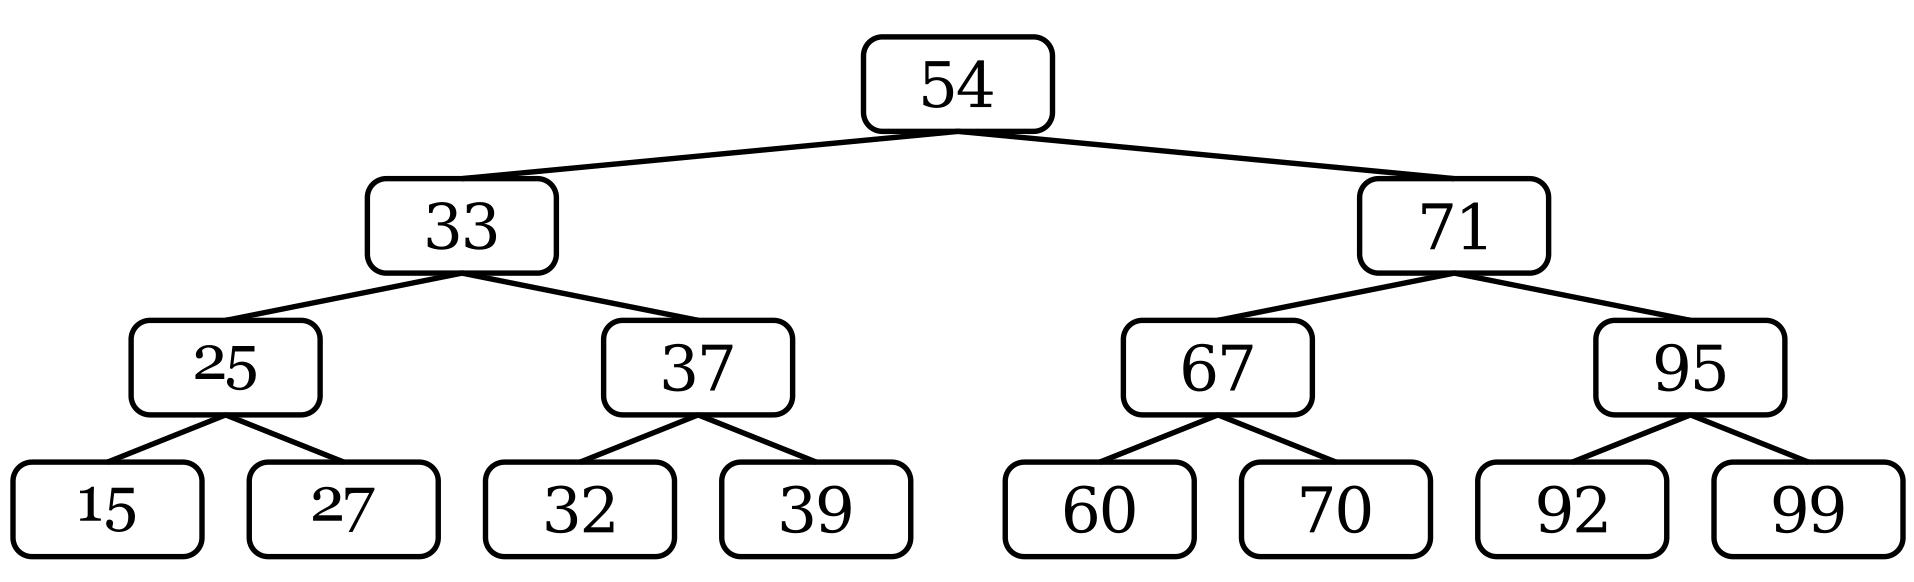
\includegraphics[scale=0.2]{../media/traversal_task.png}
\end{center}
\end{task}
\begin{task}{zur Implementierung}
Modifizieren Sie die Implementierung so, dass die Reihenfolge in einem String gespeichert wird, der am Ende zurückgegeben wird. 
\end{task}
\begin{task}{für Experten mit Langeweile}
Entwickeln Sie einen Algorithmus, der aus einer gegebenen Post-Order- und In-Order-Reihenfolge die eindeutige Struktur des binären Baumes wiederherstellt. 
\end{task}

\newpage 
\subsection{Wörterbuch mit Kompositum}

Um die vielen Null-Abfragen zu vermeiden, kann auch für die Baum-Implementierung die Baumstruktur mit Daten- und Endknoten verwendet werden. Ziel dieses Abschnitts ist es, ein erweiterbares Wörterbuch mit Hilfe der Baumstruktur zu entwickeln. Jeder Datenknoten soll dazu neben seinem Schlüssel (das englische Wort) auch eine Übersetzung enthalten (das zugehörige deutsche Wort). Anstelle der Integer, sollen jetzt also Strings in den einzelnen Datenknoten gespeichert werden. \\
\textit{Hinweis:} Auch hier könnte wieder eine Datenelement-Oberklasse (oder Interface) definiert werden. Auf diese allgemeingültige Implementierung verzichten wir hier, da das gesteckte Ziel dies nicht notwendig macht.  \\
\textbf{Randnotiz:} Mit dieser Zielsetzung hat sich auch der grundlegende Verwendungszweck unseres Baumes verändert. Im vorherigen Kapitel konnte mit dem Baum bestimmt werden, ob ein bestimmtes Element in der schon eingefügten Menge aus Zahlen vorhanden ist. Dieselbe Idee werden wir hier beim Einfügen zwar auch verwenden (es soll kein Wort im Wörterbuch doppelt vorhanden sein!), allerdings wird sich die eigentliche Benutzung verändern. \\
Das eingefügte Wort an sich ist nur ein Schlüssel, mit dem wir den eigentlichen Wert - das übersetzte Wort - finden und dann zurückgeben können. Wir stellen mit diesem Baum also eine Zuordnung her:
\begin{center}
    englisches Wort $\mapsto$ deutsches Wort
\end{center}
Im Englischen würde man hier von \textit{map} - also abbilden/zuordnen - sprechen. Entsprechend gibt es auch hier in Java bereits ein passendes \href{https://docs.oracle.com/javase/8/docs/api/java/util/Map.html}{Interface}.

\begin{task}{1}
    Implementieren Sie die notwendige Grundstruktur für das Wörterbuch mit Hilfe des Entwurfsmusters Kompositum, inklusive der einfügen-Methode (insert).
\end{task}

Die Lösung folgt hier direkt im Anschluss, keine Überraschungen in der Baum-Klasse:
\begin{minted}{Java}
    //class BinarySearchTree 
    public class BinarySearchTree {

        private Node root;

        public BinarySearchTree(){
            root = new EndNode;
        }

        public void insert(String word, String translation) {
            root = root.insert(word, translation);
        }
    }
\end{minted}

Die abstrakte Knoten-Klasse (Interface auch möglich!) enthält bisher nur Helfer-Methoden und die insert-Methode:

\begin{minted}{Java}
    //class Node 
    public abstract class Node {

        public abstract Node insert(String word, String translation);
        public abstract Node getLeft();
        public abstract Node getRight();
        public abstract void setLeft(Node n);
        public abstract void setRight(Node n);
    }
\end{minted}

Ein Datenknoten enthält drei Referenzen, auf sein linkes Kind, das rechte Kind und die beiden Datenstrings (Die Implementierungen der getter und setter fehlen im Folgenden). Das einzig interessante an der insert-Methode ist die Verwendung der bereits eingebauten compareTo()-Methode (\url{https://docs.oracle.com/javase/7/docs/api/java/lang/String.html}). Sie vergleicht die beiden Strings lexigographisch (genau das, was wir hier machen wollen) und gibt einen positiven Wert zurück, wenn der zu vergleichende String größer ist, ansonsten einen kleineren Wert. Unglücklicherweise mischt die compareTo-Methode Groß- und Kleinbuchstaben nicht, sodass wir uns auf Kleinbuchstaben als Anfang beschränken müssten. (Wählt man als Ausgangssprache Englisch und als Zielsprache Deutsch, so würde dies  keine große Einschränkung darstellen). Verwendet man alternativ die Methode compareToIgnoreCase, so hat man das Problem nicht, da \q{apple} genau wie \q{Apple} interpretiert wird und damit auch die Vergleiche entsprechende Werte liefern. 
\begin{minted}{Java}
    //class DataNode 
    public class DataNode extends Node {

        private Node left;
        private Node right;
        private String word;
        private String translation;

        public DataNode(String word, String translation) {
            this.word = word;
            this.translation = translation;
            left = new EndNode();
            right = new EndNode();
        }

        public Node insert(String word, String translation) {
            if(this.word.equals(word)) {
                System.out.println("The word is already present in the dictionary!");
                return this;
            }
            if(this.word.compareToIgnoreCase(word) < 0)  {
                right = right.insert(word, translation);
            } else {
                left = left.insert(word,translation);
            }
            return this;
        }
    }
\end{minted}

Und zuletzt in der Endknoten-Klasse:
\begin{minted}{Java}
    //class EndNode 
    public class EndNode extends Node {

        public Node insert(String word, String translation) {
            return new DataNode(word, translation);
        }
    }
\end{minted}

Diese Struktur muss nun natürlich erweitert werden. Versuchen Sie sich zunächst selbst an den folgenden Aufgaben, die Lösungen dazu finden sich im Anschluss:

\begin{task}{2}
Implementieren Sie eine übersetzen-Methode (translate), die das gegebene Wort sucht und die zugehörige Übersetzung zurückgibt. 
\end{task}

\begin{task}{3}
Implementieren Sie eine enthält-Methode (contains), die prüft, ob ein gegebenes Wort schon im Wörterbuch vorhanden ist. 
\end{task}

\begin{task}{4}
Schreiben Sie eine Methode print, die den Baum in Pre, In- und Post-Order traversieren kann. Bauen Sie einen geeigneten \q{Schalter} ein. Die Ausgabe soll auf der Konsole erfolgen. \\
Bonus: Geben Sie jeden Knoten in einer eigenen Zeile aus und rücken Sie für jede Ebene ein Leerzeichen weiter ein. 
\end{task}

\begin{task}{5}
Schreiben Sie die Methode maxTiefeGeben (maxDepth), die die maximale Tiefe des Suchbaums ausgibt. \\
\textit{Hinweis:} Verwenden Sie die Math.max()-Funktion. \\
Erweitern Sie Funktionalität, indem zusätzlich (in eigenen Methoden) die Tiefe eines bestimmten Wortes bestimmt werden kann, sowie die durchschnittlichee Tiefe aller Datenknoten des Suchbaums. 
\end{task}

\begin{task}{6}
Damit ein Suchbaum möglichst effizient ist, sollte er möglichst voll besetzt und damit balanciert sein. Ein einfaches, aber recht effizientes Kriterium dafür ist, dass die vorletzte noch besetzte Ebene bereits voll ist. Implementieren Sie eine Methode nahezuOptimal (almostOptimal), die prüft, ob dies der Fall ist. Nutzen Sie dazu die Methode, die die maximale Tiefe prüft und ergänzen Sie eine weiter Helfermethode, die die Anzahl der Knoten einer bestimmten Ebene zählt. 
\end{task}

\begin{task}{7 - Diagrammübungen}
\textbf{a) } Zeichnen Sie ein Klassendiagramm der Suchbaum-Implementierung des Wörterbuchs mit allen bisher verwendeten Methoden. \\
\textbf{b)} Zeichnen Sie einen Suchbaum, indem Sie die Wörter milk - fish - soup - rail - rest - zoo - apple - grape - dog händisch nacheinander einfügen. \\ 
\textbf{c)} Skizzieren Sie  ein Objektdiagramm für den Baum aus b) \\
\textbf{d)} Zeichnen Sie ein Sequenzdiagramm für den Baum aus b) und den Methodenaufruf maxTiefeGeben auf dem Suchbaum-Objekt. 
\end{task}

\begin{task}{8 - Für Experten}
Implementieren Sie eine Methode, die einen bestimmten Eintrag löscht. Beachten Sie dabei die Hinweise aus dem vorhergehenden Kapitel. 
\end{task}

\begin{task}{9 - Für Experten}
Invertieren Sie den Baum, d.h. an jedem Knoten soll jeweils der linke und der rechte Nachbar getauscht werden. 
\end{task}



\newpage 

\textbf{Lösungen Aufgaben} \\
\textit{Hinweis:} Im Folgenden wird die Definition der abstrakten Methoden in der Knoten-Klasse weggelassen und jeweils nur die Datenknoten bzw. Endknotenimplementierungen angegeben. \\
Wie immer beginnt in der Suchbaum-Klasse lediglich die Rekursion:
\begin{minted}{Java}
    //class BinarySearchTree
    public String translate(String word) {
        return root.translate(word);
    }
\end{minted}
Auf einem Datenknoten aufgerufen, muss zuerst überprüft werden, ob das Wort gefunden worden ist, d.h. mit dem (Schlüssel-)Wort in diesem Knoten übereinstimmt. Falls dies der Fall ist, wird die Übersetzung zurückgegeben. Andernfalls wird die Rekursion auf dem rechten Nachbarn forgesetzt, falls das Wort lexigographisch größer ist, sonst auf dem linken Kind. \\
Der Abschluss wiederum könnte einfach kein Wort zurückgeben (also einen leeren String), ich habe mich hier für den String \q{404} entschieden :).
\begin{minted}{Java}
    //class DataNode 
    @Override
    public String translate(String word) {
        if(this.word.equals(word)) {
            return translation;
        } else if(this.word.compareToIgnoreCase(word) < 0) {
            return right.translate(word);
        } else {
            return left.translate(word);
        }
    }

    //class EndNode 
    @Override
    public String translate(String word) {
        return "404";
    }
\end{minted}

Die enthält-Methode sieht fast identisch zur translate-Methode aus, nur wird bei einem gefundenen Wort \q{wahr} statt der Übersetzung zurückgegeben, der Abschluss gibt \q{falsch} zurück. 
\begin{minted}{Java}
    //class BinarySearchTree
    public boolean contains(String word) {
        return root.contains(word);
    }

    //class DataNode 
    @Override
    public boolean contains(String word) {
        if(this.word.equals(word)) {
           return true;
        }
        if(this.word.compareToIgnoreCase(word) < 0)  {
            return right.contains(word);
        } else {
            return left.contains(word);
        }
    }

    //class EndNode
    @Override 
    public boolean contains(String word) {
        return false;
    }
\end{minted}
Die erste Variante der print-Methode kann nahezu identisch aus dem vorherigen Kapitel übernommen werden (lediglich der Variablenname muss angepasst werden und ein Endknoten muss die Rekursion beenden):
\begin{minted}{Java}
    //class BinarySearchTree
    public void print(Order order) {
        root.print(order);
    }

    //enum Order
    public enum Order {
        PRE,
        POST, 
        IN
    }

    //class DataNode 
    @Override 
    public void print(Order order) {
        if(order == Order.PRE) System.out.print(word + " ");
        left.print(order);
        if(order == Order.IN) System.out.print(word + " ");
        right.print(order);
        if(order == Order.POST) System.out.print(word + " ");
    }

    //class EndNode
    @Override 
    public void print(Order order) {
        return;
    }
\end{minted}
Für die Einrückung ist es am leichtesten einen weiteren Übergabeparameter \q{einrückung} (indent) zu definieren, der bei jedem Aufruf ein Doppelleerzeichen (beliebig, könnten auch mehr sein oder nur eines!) mehr anhängt:
\begin{minted}{Java}
    //class BinarySearchTree
    public void printIndent(Order order) {
        root.printIndent(order, "");
    }

    //class DataNode
    @Override 
    public void printIndent(Order order, String indent) {
        if(order == Order.PRE) System.out.println(indent + word);
        left.printIndent(order, indent + "  ");
        if(order == Order.IN) System.out.println(indent + word);
        right.printIndent(order, indent + "  ");
        if(order == Order.POST) System.out.println(indent + word);
    }

    //class EndNode 
    @Override 
    public void printIndent(Order order, String indent) {
        return;
    }
\end{minted}
Die fünfte Aufgabe ist recht umfangreich, beginnen wir mit der maximalen Tiefe. Die grundlegende Idee besteht darin, in jedem Schritt der Rekursion die Methode auf beiden Teilbäumen aufzurufen, allerdings nur den größeren der beiden Werte weiterzugeben. Hier kommt die Math.max() Funktion ins Spiel, die uns genau den größeren der beiden Werte auswählt. \\
\textit{Hinweis:} Natürlich kann man sich auch eine \q{eigene} max()-Funktion definieren. \\
Der Endknoten bricht natürlich wieder ab, indem er 0 zurückgibt. 
\begin{minted}{Java}
    //class BinarySearchTree
    public int maxDepth() {
        return root.maxDepth();
    }

    //class DataNode 
    @Override 
    public int maxDepth() {
        return Math.max(left.maxDepth() + 1, right.maxDepth() + 1);
    }

    //class EndNode 
    @Override 
    public int maxDepth() {
        return 0;
    }
\end{minted}
Für die Tiefe eines Wortes kann wieder dieselbe Logik wie bei der übersetzen-Methode verwendet werden, nur zählen wir jetzt jeden Schritt mit und geben am Ende die gegangenen Schritte zurück, statt der Übersetzung:
\begin{minted}{Java}
    //class BinarySearchTree
    public int depthOf(String word) {
        return root.depthOf(word, 1);
    }

    //class DataNode 
    @Override 
    public int depthOf(String word, int counter) {
        if(this.word.equals(word)) {
            return counter;
        } else if(this.word.compareToIgnoreCase(word) < 0) {
            return right.depthOf(word, counter + 1);
        } else {
            return left.depthOf(word, counter + 1);
        }
    } 

    //class EndNode 
    @Override 
    public int depthOf(String word, int counter) {
        return 0;
    }
\end{minted}
Die durchschnittliche Tiefe eines Knotens erfordert ein wenig mehr Arbeit. Die grundlegende Idee liegt darin, zuerst alle Knoten zu zählen (das könnte man natürlich auch über ein Attribut beim Einfügen lösen, ähnlich wie bei der Liste). Dann summiert man die Tiefen aller Knoten und teilt sie abschließend durch die Anzahl. Diese \q{Tiefensummen}-Funktion addiert immer die aktuelle Tiefe des Knotens auf die Ergebnisse der Funktionsaufrufe auf den beiden Kindern. \\
Im Code sieht das dann so aus:
\begin{minted}{Java}
    //class BinarySearchTree 
    public double averageDepth() {
       double n = (double) numberOfNodes();
       if(n > 0) {
            return sumOfDepths()/n;
       }
       return 0;
    }

    public int numberOfNodes() {
        return root.numberOfNodes();
    }

    public int sumOfDepths() {
        return root.sumOfDepths(1);
    }
\end{minted}
Da insbesondere das Zählen der Knoten auch in einem anderen Kontext nützlich sein könnte, wurde es in eine eigene Methode ausgelagert, ebenso wie die Tiefensummen-Methode. Für die Erfüllung der Aufgabe wäre eine \q{große} Methode aber auch in Ordnung. 
\begin{minted}{Java}
    //class DataNode 
    @Override 
    public int numberOfNodes() {
        return left.numberOfNodes() + right.numberOfNodes() + 1;
    }

    @Override 
    public int sumOfDepths(int currentDepth) {
        System.out.println(currentDepth);
        return currentDepth + left.sumOfDepths(currentDepth + 1) + right.sumOfDepths(currentDepth + 1);
    }

    //class EndNode 
    @Override 
    public int numberOfNodes() {
        return 0;
    }

    @Override 
    public int sumOfDepths(int currentDepth) {
        return 0;
    }
\end{minted}
Die Implementierung der Methode, die prüft, ob die vorletzte Ebene des Baumes bestzt ist, beginnt wie folgt: 
\begin{minted}{Java}
    //class BinarySearchTree
    public boolean almostOptimal() {
        int d = maxDepth();
        if(d <= 2) {
            return true;
        }
        double targetNumber = Math.pow(2, d - 2);
        double actualNumber = (double) sumInRow(d - 1);
        if(targetNumber == actualNumber) {
            return true;
        } else {
            return false;
        }
    }
\end{minted}
$d$ gibt die Tiefe unseres Baumes an, ist diese kleiner oder gleich 2, so ist der Baum in jedem Fall optimal (im Fall der Tiefe 2 müsste nur die Existenz der Wurzel geprüft werden, diese ist immer vorhanden!). \\
Falls $d$ dagegen größer ist als 2, so müssen in der Reihe $d-1$ genau $2^{d-2}$ Knoten sein. Folgendes Bild veranschaulicht dies: 
\begin{center}
    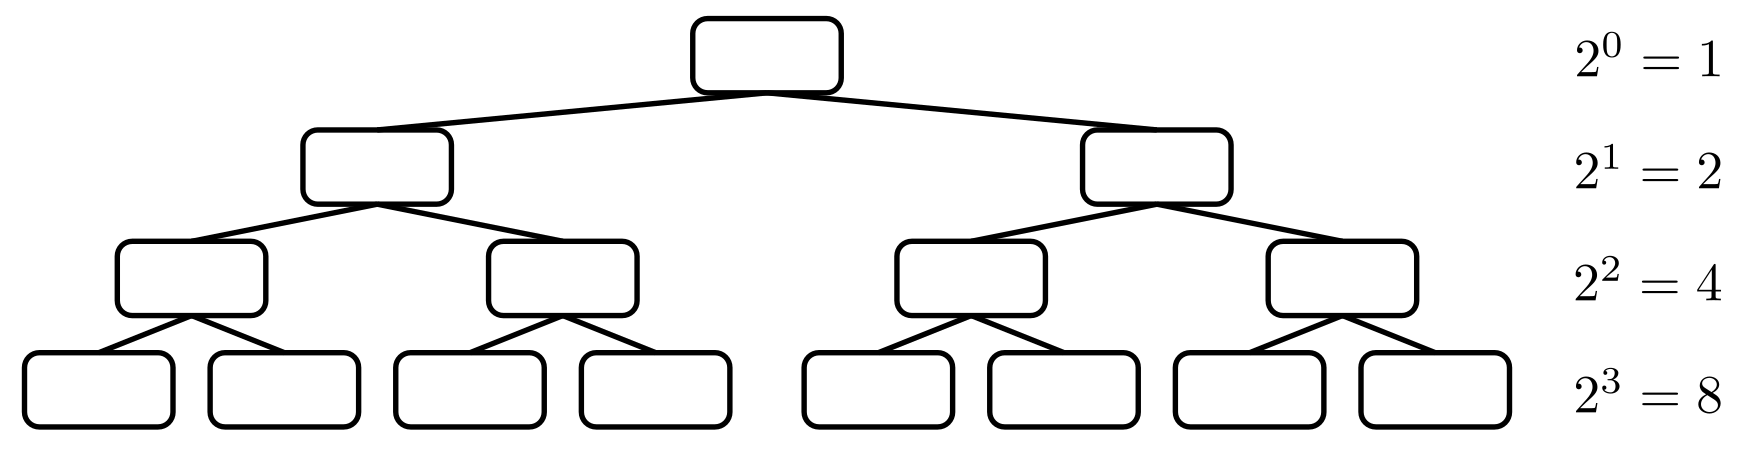
\includegraphics[scale=0.25]{../media/number_nodes.png}
\end{center}
Die rekursive Helfer-Methode summeInEinerEbene funktioniert wieder ähnlich wie die übrigens rekursiven Methoden: 
\begin{minted}{Java}
    //class BinarySearchTree
    public int sumInRow(int depth) {
        return root.sumInRow(depth);
    }

    //class DataNode 
    @Override 
    public int sumInRow(int depth) {
        if(depth == 1) return 1;
        return left.sumInRow(depth - 1) + right.sumInRow(depth - 1);
    } 

    //class EndNode 
    @Override 
    public int sumInRow(int depth) {
        return 0;
    }
\end{minted}

\end{document}